% Created by tikzDevice version 0.12.3.1 on 2021-12-15 17:50:48
% !TEX encoding = UTF-8 Unicode
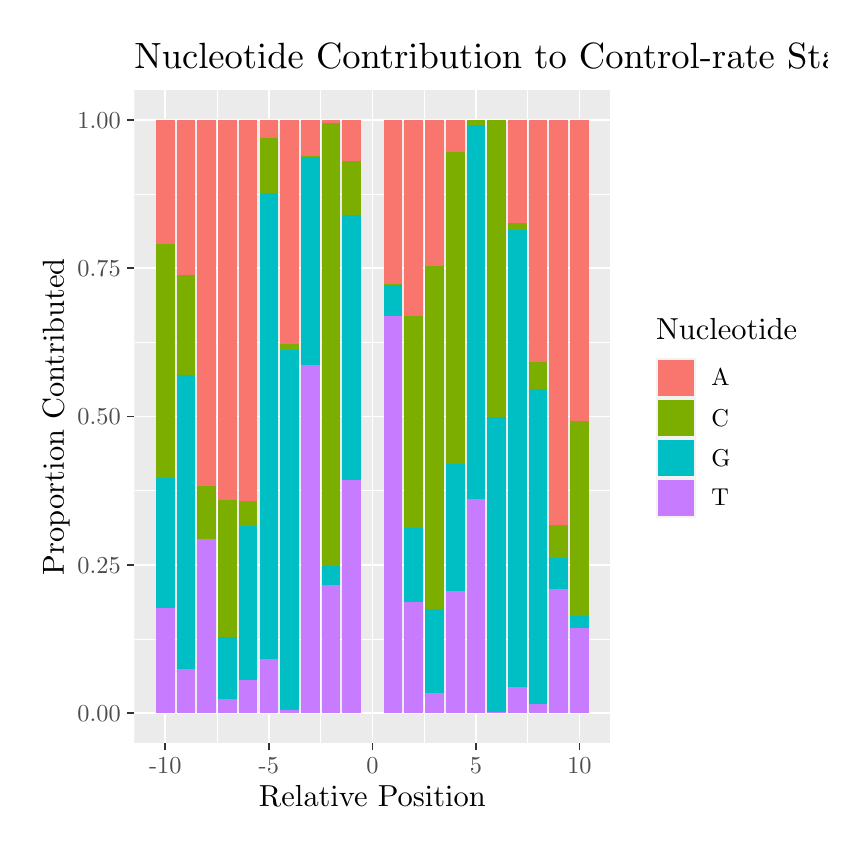
\begin{tikzpicture}[x=1pt,y=1pt]
\definecolor{fillColor}{RGB}{255,255,255}
\path[use as bounding box,fill=fillColor,fill opacity=0.00] (0,0) rectangle (289.08,289.08);
\begin{scope}
\path[clip] (  0.00,  0.00) rectangle (289.08,289.08);
\definecolor{drawColor}{RGB}{255,255,255}
\definecolor{fillColor}{RGB}{255,255,255}

\path[draw=drawColor,line width= 0.6pt,line join=round,line cap=round,fill=fillColor] (  0.00,  0.00) rectangle (289.08,289.08);
\end{scope}
\begin{scope}
\path[clip] ( 38.56, 30.69) rectangle (210.56,266.42);
\definecolor{fillColor}{gray}{0.92}

\path[fill=fillColor] ( 38.56, 30.69) rectangle (210.56,266.42);
\definecolor{drawColor}{RGB}{255,255,255}

\path[draw=drawColor,line width= 0.3pt,line join=round] ( 38.56, 68.19) --
	(210.56, 68.19);

\path[draw=drawColor,line width= 0.3pt,line join=round] ( 38.56,121.77) --
	(210.56,121.77);

\path[draw=drawColor,line width= 0.3pt,line join=round] ( 38.56,175.34) --
	(210.56,175.34);

\path[draw=drawColor,line width= 0.3pt,line join=round] ( 38.56,228.92) --
	(210.56,228.92);

\path[draw=drawColor,line width= 0.3pt,line join=round] ( 68.45, 30.69) --
	( 68.45,266.42);

\path[draw=drawColor,line width= 0.3pt,line join=round] (105.85, 30.69) --
	(105.85,266.42);

\path[draw=drawColor,line width= 0.3pt,line join=round] (143.26, 30.69) --
	(143.26,266.42);

\path[draw=drawColor,line width= 0.3pt,line join=round] (180.67, 30.69) --
	(180.67,266.42);

\path[draw=drawColor,line width= 0.6pt,line join=round] ( 38.56, 41.40) --
	(210.56, 41.40);

\path[draw=drawColor,line width= 0.6pt,line join=round] ( 38.56, 94.98) --
	(210.56, 94.98);

\path[draw=drawColor,line width= 0.6pt,line join=round] ( 38.56,148.55) --
	(210.56,148.55);

\path[draw=drawColor,line width= 0.6pt,line join=round] ( 38.56,202.13) --
	(210.56,202.13);

\path[draw=drawColor,line width= 0.6pt,line join=round] ( 38.56,255.71) --
	(210.56,255.71);

\path[draw=drawColor,line width= 0.6pt,line join=round] ( 49.74, 30.69) --
	( 49.74,266.42);

\path[draw=drawColor,line width= 0.6pt,line join=round] ( 87.15, 30.69) --
	( 87.15,266.42);

\path[draw=drawColor,line width= 0.6pt,line join=round] (124.56, 30.69) --
	(124.56,266.42);

\path[draw=drawColor,line width= 0.6pt,line join=round] (161.97, 30.69) --
	(161.97,266.42);

\path[draw=drawColor,line width= 0.6pt,line join=round] (199.38, 30.69) --
	(199.38,266.42);
\definecolor{fillColor}{RGB}{248,118,109}

\path[fill=fillColor] ( 46.37,210.99) rectangle ( 53.11,255.71);
\definecolor{fillColor}{RGB}{124,174,0}

\path[fill=fillColor] ( 46.37,126.35) rectangle ( 53.11,210.99);
\definecolor{fillColor}{RGB}{0,191,196}

\path[fill=fillColor] ( 46.37, 79.51) rectangle ( 53.11,126.35);
\definecolor{fillColor}{RGB}{199,124,255}

\path[fill=fillColor] ( 46.37, 41.40) rectangle ( 53.11, 79.51);
\definecolor{fillColor}{RGB}{248,118,109}

\path[fill=fillColor] ( 53.86,199.56) rectangle ( 60.59,255.71);
\definecolor{fillColor}{RGB}{124,174,0}

\path[fill=fillColor] ( 53.86,163.62) rectangle ( 60.59,199.56);
\definecolor{fillColor}{RGB}{0,191,196}

\path[fill=fillColor] ( 53.86, 57.39) rectangle ( 60.59,163.62);
\definecolor{fillColor}{RGB}{199,124,255}

\path[fill=fillColor] ( 53.86, 41.40) rectangle ( 60.59, 57.39);
\definecolor{fillColor}{RGB}{248,118,109}

\path[fill=fillColor] ( 61.34,123.58) rectangle ( 68.07,255.71);
\definecolor{fillColor}{RGB}{124,174,0}

\path[fill=fillColor] ( 61.34,104.38) rectangle ( 68.07,123.58);
\definecolor{fillColor}{RGB}{0,191,196}

\path[fill=fillColor] ( 61.34,104.26) rectangle ( 68.07,104.38);
\definecolor{fillColor}{RGB}{199,124,255}

\path[fill=fillColor] ( 61.34, 41.40) rectangle ( 68.07,104.26);
\definecolor{fillColor}{RGB}{248,118,109}

\path[fill=fillColor] ( 68.82,118.36) rectangle ( 75.55,255.71);
\definecolor{fillColor}{RGB}{124,174,0}

\path[fill=fillColor] ( 68.82, 69.00) rectangle ( 75.55,118.36);
\definecolor{fillColor}{RGB}{199,124,255}

\path[fill=fillColor] ( 68.82, 41.40) rectangle ( 75.55, 46.34);
\definecolor{fillColor}{RGB}{0,191,196}

\path[fill=fillColor] ( 68.82, 46.34) rectangle ( 75.55, 69.00);
\definecolor{fillColor}{RGB}{248,118,109}

\path[fill=fillColor] ( 76.30,118.00) rectangle ( 83.04,255.71);
\definecolor{fillColor}{RGB}{124,174,0}

\path[fill=fillColor] ( 76.30,108.86) rectangle ( 83.04,118.00);
\definecolor{fillColor}{RGB}{0,191,196}

\path[fill=fillColor] ( 76.30, 53.22) rectangle ( 83.04,108.86);
\definecolor{fillColor}{RGB}{199,124,255}

\path[fill=fillColor] ( 76.30, 41.40) rectangle ( 83.04, 53.22);
\definecolor{fillColor}{RGB}{248,118,109}

\path[fill=fillColor] ( 83.78,249.36) rectangle ( 90.52,255.71);
\definecolor{fillColor}{RGB}{124,174,0}

\path[fill=fillColor] ( 83.78,229.34) rectangle ( 90.52,249.36);
\definecolor{fillColor}{RGB}{0,191,196}

\path[fill=fillColor] ( 83.78, 60.85) rectangle ( 90.52,229.34);
\definecolor{fillColor}{RGB}{199,124,255}

\path[fill=fillColor] ( 83.78, 41.40) rectangle ( 90.52, 60.85);
\definecolor{fillColor}{RGB}{248,118,109}

\path[fill=fillColor] ( 91.27,174.63) rectangle ( 98.00,255.71);
\definecolor{fillColor}{RGB}{124,174,0}

\path[fill=fillColor] ( 91.27,172.60) rectangle ( 98.00,174.63);
\definecolor{fillColor}{RGB}{0,191,196}

\path[fill=fillColor] ( 91.27, 42.65) rectangle ( 98.00,172.60);
\definecolor{fillColor}{RGB}{199,124,255}

\path[fill=fillColor] ( 91.27, 41.40) rectangle ( 98.00, 42.65);
\definecolor{fillColor}{RGB}{248,118,109}

\path[fill=fillColor] ( 98.75,242.70) rectangle (105.48,255.71);
\definecolor{fillColor}{RGB}{124,174,0}

\path[fill=fillColor] ( 98.75,242.52) rectangle (105.48,242.70);
\definecolor{fillColor}{RGB}{199,124,255}

\path[fill=fillColor] ( 98.75, 41.40) rectangle (105.48,167.08);
\definecolor{fillColor}{RGB}{0,191,196}

\path[fill=fillColor] ( 98.75,167.08) rectangle (105.48,242.52);
\definecolor{fillColor}{RGB}{248,118,109}

\path[fill=fillColor] (106.23,254.78) rectangle (112.96,255.71);
\definecolor{fillColor}{RGB}{124,174,0}

\path[fill=fillColor] (106.23, 94.57) rectangle (112.96,254.78);
\definecolor{fillColor}{RGB}{199,124,255}

\path[fill=fillColor] (106.23, 41.40) rectangle (112.96, 87.57);
\definecolor{fillColor}{RGB}{0,191,196}

\path[fill=fillColor] (106.23, 87.57) rectangle (112.96, 94.57);
\definecolor{fillColor}{RGB}{248,118,109}

\path[fill=fillColor] (113.71,240.77) rectangle (120.44,255.71);
\definecolor{fillColor}{RGB}{124,174,0}

\path[fill=fillColor] (113.71,221.55) rectangle (120.44,240.77);
\definecolor{fillColor}{RGB}{0,191,196}

\path[fill=fillColor] (113.71,125.62) rectangle (120.44,221.55);
\definecolor{fillColor}{RGB}{199,124,255}

\path[fill=fillColor] (113.71, 41.40) rectangle (120.44,125.62);
\definecolor{fillColor}{RGB}{248,118,109}

\path[fill=fillColor] (128.67,196.59) rectangle (135.41,255.71);
\definecolor{fillColor}{RGB}{124,174,0}

\path[fill=fillColor] (128.67,196.15) rectangle (135.41,196.59);
\definecolor{fillColor}{RGB}{0,191,196}

\path[fill=fillColor] (128.67,185.01) rectangle (135.41,196.15);
\definecolor{fillColor}{RGB}{199,124,255}

\path[fill=fillColor] (128.67, 41.40) rectangle (135.41,185.01);
\definecolor{fillColor}{RGB}{248,118,109}

\path[fill=fillColor] (136.16,184.73) rectangle (142.89,255.71);
\definecolor{fillColor}{RGB}{124,174,0}

\path[fill=fillColor] (136.16,108.46) rectangle (142.89,184.73);
\definecolor{fillColor}{RGB}{0,191,196}

\path[fill=fillColor] (136.16, 81.69) rectangle (142.89,108.46);
\definecolor{fillColor}{RGB}{199,124,255}

\path[fill=fillColor] (136.16, 41.40) rectangle (142.89, 81.69);
\definecolor{fillColor}{RGB}{248,118,109}

\path[fill=fillColor] (143.64,203.11) rectangle (150.37,255.71);
\definecolor{fillColor}{RGB}{124,174,0}

\path[fill=fillColor] (143.64, 79.18) rectangle (150.37,203.11);
\definecolor{fillColor}{RGB}{199,124,255}

\path[fill=fillColor] (143.64, 41.40) rectangle (150.37, 48.64);
\definecolor{fillColor}{RGB}{0,191,196}

\path[fill=fillColor] (143.64, 48.64) rectangle (150.37, 79.18);
\definecolor{fillColor}{RGB}{248,118,109}

\path[fill=fillColor] (151.12,244.13) rectangle (157.85,255.71);
\definecolor{fillColor}{RGB}{124,174,0}

\path[fill=fillColor] (151.12,131.59) rectangle (157.85,244.13);
\definecolor{fillColor}{RGB}{0,191,196}

\path[fill=fillColor] (151.12, 85.53) rectangle (157.85,131.59);
\definecolor{fillColor}{RGB}{199,124,255}

\path[fill=fillColor] (151.12, 41.40) rectangle (157.85, 85.53);
\definecolor{fillColor}{RGB}{248,118,109}

\path[fill=fillColor] (158.60,255.64) rectangle (165.34,255.71);
\definecolor{fillColor}{RGB}{124,174,0}

\path[fill=fillColor] (158.60,254.01) rectangle (165.34,255.64);
\definecolor{fillColor}{RGB}{0,191,196}

\path[fill=fillColor] (158.60,118.89) rectangle (165.34,254.01);
\definecolor{fillColor}{RGB}{199,124,255}

\path[fill=fillColor] (158.60, 41.40) rectangle (165.34,118.89);
\definecolor{fillColor}{RGB}{248,118,109}

\path[fill=fillColor] (166.08,255.69) rectangle (172.82,255.71);
\definecolor{fillColor}{RGB}{124,174,0}

\path[fill=fillColor] (166.08,148.35) rectangle (172.82,255.69);
\definecolor{fillColor}{RGB}{199,124,255}

\path[fill=fillColor] (166.08, 41.40) rectangle (172.82, 41.65);
\definecolor{fillColor}{RGB}{0,191,196}

\path[fill=fillColor] (166.08, 41.65) rectangle (172.82,148.35);
\definecolor{fillColor}{RGB}{248,118,109}

\path[fill=fillColor] (173.57,218.65) rectangle (180.30,255.71);
\definecolor{fillColor}{RGB}{124,174,0}

\path[fill=fillColor] (173.57,216.11) rectangle (180.30,218.65);
\definecolor{fillColor}{RGB}{199,124,255}

\path[fill=fillColor] (173.57, 41.40) rectangle (180.30, 50.99);
\definecolor{fillColor}{RGB}{0,191,196}

\path[fill=fillColor] (173.57, 50.99) rectangle (180.30,216.11);
\definecolor{fillColor}{RGB}{248,118,109}

\path[fill=fillColor] (181.05,168.43) rectangle (187.78,255.71);
\definecolor{fillColor}{RGB}{124,174,0}

\path[fill=fillColor] (181.05,158.47) rectangle (187.78,168.43);
\definecolor{fillColor}{RGB}{0,191,196}

\path[fill=fillColor] (181.05, 44.71) rectangle (187.78,158.47);
\definecolor{fillColor}{RGB}{199,124,255}

\path[fill=fillColor] (181.05, 41.40) rectangle (187.78, 44.71);
\definecolor{fillColor}{RGB}{248,118,109}

\path[fill=fillColor] (188.53,109.43) rectangle (195.26,255.71);
\definecolor{fillColor}{RGB}{124,174,0}

\path[fill=fillColor] (188.53, 97.48) rectangle (195.26,109.43);
\definecolor{fillColor}{RGB}{0,191,196}

\path[fill=fillColor] (188.53, 86.28) rectangle (195.26, 97.48);
\definecolor{fillColor}{RGB}{199,124,255}

\path[fill=fillColor] (188.53, 41.40) rectangle (195.26, 86.28);
\definecolor{fillColor}{RGB}{248,118,109}

\path[fill=fillColor] (196.01,147.09) rectangle (202.75,255.71);
\definecolor{fillColor}{RGB}{124,174,0}

\path[fill=fillColor] (196.01, 76.62) rectangle (202.75,147.09);
\definecolor{fillColor}{RGB}{0,191,196}

\path[fill=fillColor] (196.01, 72.01) rectangle (202.75, 76.62);
\definecolor{fillColor}{RGB}{199,124,255}

\path[fill=fillColor] (196.01, 41.40) rectangle (202.75, 72.01);
\end{scope}
\begin{scope}
\path[clip] (  0.00,  0.00) rectangle (289.08,289.08);
\definecolor{drawColor}{gray}{0.30}

\node[text=drawColor,anchor=base east,inner sep=0pt, outer sep=0pt, scale=  0.88] at ( 33.61, 38.37) {0.00};

\node[text=drawColor,anchor=base east,inner sep=0pt, outer sep=0pt, scale=  0.88] at ( 33.61, 91.95) {0.25};

\node[text=drawColor,anchor=base east,inner sep=0pt, outer sep=0pt, scale=  0.88] at ( 33.61,145.52) {0.50};

\node[text=drawColor,anchor=base east,inner sep=0pt, outer sep=0pt, scale=  0.88] at ( 33.61,199.10) {0.75};

\node[text=drawColor,anchor=base east,inner sep=0pt, outer sep=0pt, scale=  0.88] at ( 33.61,252.68) {1.00};
\end{scope}
\begin{scope}
\path[clip] (  0.00,  0.00) rectangle (289.08,289.08);
\definecolor{drawColor}{gray}{0.20}

\path[draw=drawColor,line width= 0.6pt,line join=round] ( 35.81, 41.40) --
	( 38.56, 41.40);

\path[draw=drawColor,line width= 0.6pt,line join=round] ( 35.81, 94.98) --
	( 38.56, 94.98);

\path[draw=drawColor,line width= 0.6pt,line join=round] ( 35.81,148.55) --
	( 38.56,148.55);

\path[draw=drawColor,line width= 0.6pt,line join=round] ( 35.81,202.13) --
	( 38.56,202.13);

\path[draw=drawColor,line width= 0.6pt,line join=round] ( 35.81,255.71) --
	( 38.56,255.71);
\end{scope}
\begin{scope}
\path[clip] (  0.00,  0.00) rectangle (289.08,289.08);
\definecolor{drawColor}{gray}{0.20}

\path[draw=drawColor,line width= 0.6pt,line join=round] ( 49.74, 27.94) --
	( 49.74, 30.69);

\path[draw=drawColor,line width= 0.6pt,line join=round] ( 87.15, 27.94) --
	( 87.15, 30.69);

\path[draw=drawColor,line width= 0.6pt,line join=round] (124.56, 27.94) --
	(124.56, 30.69);

\path[draw=drawColor,line width= 0.6pt,line join=round] (161.97, 27.94) --
	(161.97, 30.69);

\path[draw=drawColor,line width= 0.6pt,line join=round] (199.38, 27.94) --
	(199.38, 30.69);
\end{scope}
\begin{scope}
\path[clip] (  0.00,  0.00) rectangle (289.08,289.08);
\definecolor{drawColor}{gray}{0.30}

\node[text=drawColor,anchor=base,inner sep=0pt, outer sep=0pt, scale=  0.88] at ( 49.74, 19.68) {-10};

\node[text=drawColor,anchor=base,inner sep=0pt, outer sep=0pt, scale=  0.88] at ( 87.15, 19.68) {-5};

\node[text=drawColor,anchor=base,inner sep=0pt, outer sep=0pt, scale=  0.88] at (124.56, 19.68) {0};

\node[text=drawColor,anchor=base,inner sep=0pt, outer sep=0pt, scale=  0.88] at (161.97, 19.68) {5};

\node[text=drawColor,anchor=base,inner sep=0pt, outer sep=0pt, scale=  0.88] at (199.38, 19.68) {10};
\end{scope}
\begin{scope}
\path[clip] (  0.00,  0.00) rectangle (289.08,289.08);
\definecolor{drawColor}{RGB}{0,0,0}

\node[text=drawColor,anchor=base,inner sep=0pt, outer sep=0pt, scale=  1.10] at (124.56,  7.64) {Relative Position};
\end{scope}
\begin{scope}
\path[clip] (  0.00,  0.00) rectangle (289.08,289.08);
\definecolor{drawColor}{RGB}{0,0,0}

\node[text=drawColor,rotate= 90.00,anchor=base,inner sep=0pt, outer sep=0pt, scale=  1.10] at ( 13.08,148.55) {Proportion Contributed};
\end{scope}
\begin{scope}
\path[clip] (  0.00,  0.00) rectangle (289.08,289.08);
\definecolor{fillColor}{RGB}{255,255,255}

\path[fill=fillColor] (221.56,106.54) rectangle (283.58,190.57);
\end{scope}
\begin{scope}
\path[clip] (  0.00,  0.00) rectangle (289.08,289.08);
\definecolor{drawColor}{RGB}{0,0,0}

\node[text=drawColor,anchor=base west,inner sep=0pt, outer sep=0pt, scale=  1.10] at (227.06,176.42) {Nucleotide};
\end{scope}
\begin{scope}
\path[clip] (  0.00,  0.00) rectangle (289.08,289.08);
\definecolor{fillColor}{gray}{0.95}

\path[fill=fillColor] (227.06,155.40) rectangle (241.52,169.86);
\end{scope}
\begin{scope}
\path[clip] (  0.00,  0.00) rectangle (289.08,289.08);
\definecolor{fillColor}{RGB}{248,118,109}

\path[fill=fillColor] (227.78,156.11) rectangle (240.81,169.14);
\end{scope}
\begin{scope}
\path[clip] (  0.00,  0.00) rectangle (289.08,289.08);
\definecolor{fillColor}{gray}{0.95}

\path[fill=fillColor] (227.06,140.95) rectangle (241.52,155.40);
\end{scope}
\begin{scope}
\path[clip] (  0.00,  0.00) rectangle (289.08,289.08);
\definecolor{fillColor}{RGB}{124,174,0}

\path[fill=fillColor] (227.78,141.66) rectangle (240.81,154.69);
\end{scope}
\begin{scope}
\path[clip] (  0.00,  0.00) rectangle (289.08,289.08);
\definecolor{fillColor}{gray}{0.95}

\path[fill=fillColor] (227.06,126.49) rectangle (241.52,140.95);
\end{scope}
\begin{scope}
\path[clip] (  0.00,  0.00) rectangle (289.08,289.08);
\definecolor{fillColor}{RGB}{0,191,196}

\path[fill=fillColor] (227.78,127.20) rectangle (240.81,140.24);
\end{scope}
\begin{scope}
\path[clip] (  0.00,  0.00) rectangle (289.08,289.08);
\definecolor{fillColor}{gray}{0.95}

\path[fill=fillColor] (227.06,112.04) rectangle (241.52,126.49);
\end{scope}
\begin{scope}
\path[clip] (  0.00,  0.00) rectangle (289.08,289.08);
\definecolor{fillColor}{RGB}{199,124,255}

\path[fill=fillColor] (227.78,112.75) rectangle (240.81,125.78);
\end{scope}
\begin{scope}
\path[clip] (  0.00,  0.00) rectangle (289.08,289.08);
\definecolor{drawColor}{RGB}{0,0,0}

\node[text=drawColor,anchor=base west,inner sep=0pt, outer sep=0pt, scale=  0.88] at (247.02,159.60) {A};
\end{scope}
\begin{scope}
\path[clip] (  0.00,  0.00) rectangle (289.08,289.08);
\definecolor{drawColor}{RGB}{0,0,0}

\node[text=drawColor,anchor=base west,inner sep=0pt, outer sep=0pt, scale=  0.88] at (247.02,145.14) {C};
\end{scope}
\begin{scope}
\path[clip] (  0.00,  0.00) rectangle (289.08,289.08);
\definecolor{drawColor}{RGB}{0,0,0}

\node[text=drawColor,anchor=base west,inner sep=0pt, outer sep=0pt, scale=  0.88] at (247.02,130.69) {G};
\end{scope}
\begin{scope}
\path[clip] (  0.00,  0.00) rectangle (289.08,289.08);
\definecolor{drawColor}{RGB}{0,0,0}

\node[text=drawColor,anchor=base west,inner sep=0pt, outer sep=0pt, scale=  0.88] at (247.02,116.24) {T};
\end{scope}
\begin{scope}
\path[clip] (  0.00,  0.00) rectangle (289.08,289.08);
\definecolor{drawColor}{RGB}{0,0,0}

\node[text=drawColor,anchor=base west,inner sep=0pt, outer sep=0pt, scale=  1.32] at ( 38.56,274.49) {Nucleotide Contribution to Control-rate Statistic: AT-GC};
\end{scope}
\end{tikzpicture}
